\documentclass[crop=false,a4paper,oneside,11pt]{standalone}
\usepackage{a4wide,graphicx,fancyhdr,amsmath,amssymb,float,graphicx,color,geometry,xcolor,titlesec,colortbl,tabu}
\usepackage[parfill]{parskip}
\usepackage[nodayofweek]{datetime}
\usepackage{float}
%----------------------- Macros and Definitions --------------------------

%fast change of things
\newcommand{\mysubject}{2IO90 DBL Algorithms}
\newcommand{\myassignment}{Group 4}

%\definecolor{titlepagecolor}{cmyk}{1,.60,0,.40}
%\definecolor{namecolor}{cmyk}{1,.50,0,.10}


\setlength\headheight{20pt}
\addtolength\topmargin{-10pt}
\addtolength\footskip{20pt}

% Define light and dark Microsoft blue colours
\definecolor{MSBlue}{rgb}{.204,.353,.541}
\definecolor{MSLightBlue}{rgb}{.31,.506,.741}
\arrayrulecolor{MSLightBlue}

% Set formats for each heading level

\titleformat*{\section}{\Large\bfseries\sffamily\color{MSBlue}}
\titleformat*{\subsection}{\large\bfseries\sffamily\color{MSLightBlue}}

%date format
\newdateformat{mydate}{\monthname[\THEMONTH] \THEYEAR}

\fancypagestyle{plain}{%
\fancyhf{}
\renewcommand{\headrulewidth}{0pt}
\renewcommand{\footrulewidth}{0pt}
}

\pagestyle{fancy}
\fancyhf{}
\fancyfoot[CO] {\thepage}
\renewcommand{\headrulewidth}{0pt}
\renewcommand{\footrulewidth}{0pt}


%--------------------------------- Text ----------------------------------
\setcounter{secnumdepth}{0}
\begin{document}

\begin{abstract}
The readability of maps is related to the amount of overlaps text labels have. Point-feature label placement (we use PFLP in this paper) is the problem of placing text labels next to features on a map with the goal of maximising legibility, where labels can still overlap. In our paper we focus on the PFLP problem to maximise a subset of labels that are placed without any overlap. We use the 2-position, 4-position and 1-slider models to place labels that have a fixed height and width and present algorithms for these models. In our paper we present algorithms for the 2-position, 4-position and 1-slider models with running times $O(n^2)$, $O(n^2)$ and ... respectively.
\end{abstract}

\section{Introduction}
From the earliest maps in ancient times to Google Maps today, labeling points with text on a map has always been an important and time consuming task. A cartographer can typically only place between 20 and 30 labels an hour [5], as such it becomes desirable to automate the placement of labels. In cartography there are three types of features that need to be labeled. These three are: area placement(e.g. lakes), line placement (e.g. rivers) and point placement(e.g. cities) [4]. In our paper we focus on point placement. This problem is also known as the Point-feature label placement (we shall call this PFLP in the rest of the paper) problem. The PFLP problem is about placing text labels next to all points such that it maximises readability.

 There has been much research done on variations of the Point-feature label placement problem and many of the algorithms that have been presented focus on the placing of text labels with the least amount of overlaps [2][6]. An overview of research done on automatic label placement up to 2009 can be found in the bibliography [3] that was maintained by Alexander Wolff. One of the most useful articles we found was that of Alexander Wolff, titled \emph{Automated Label Placement in Theory and Practice} [1]. Wolff describes a wide range of algorithms for different kinds of placement models and compares these against other already used algorithms. Other approaches that are used in the map-labeling problem are gradient descent or simulated annealing. J. Christensen, J. Marks and S. Shieber present methods for these in their work [2]. More recently there have been papers focusing on the PFLP problem for dynamic maps [7][8].

 In our paper we focus on algorithms that label a maximum amount of points such that there are no overlaps given a fixed height and width. These algorithms also have to terminate within a time limit of five minutes. The points have $x$- and $y$-coordinates that are integers in the range of $\left\{0,1,...,10000\right\}$.

 We use three different placement models to place the labels, see figure 1.
 \begin{enumerate}
 \item[1.] The 2-position model, where either the bottom left or the bottom right-hand corner of the labels coincide with the points.
 \item[2.] The 4-position model, where any of the corners coincide with the points.
 \item[3.] The 1-slider model, where the bottom edge of the label crosses the point and the horizontal position is determined by a so-called slider variable.
 \begin{figure}[h!]
 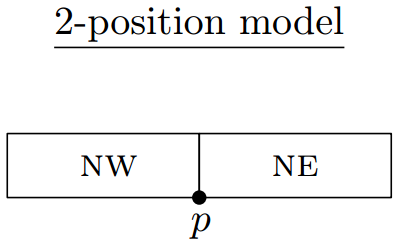
\includegraphics[scale = 0.5]{2pos.png} 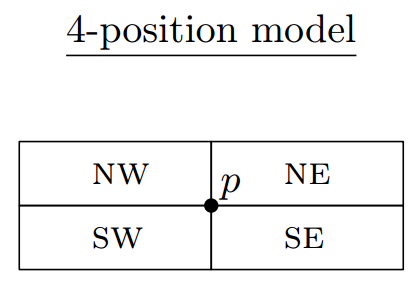
\includegraphics[scale = 0.5]{4pos.png} 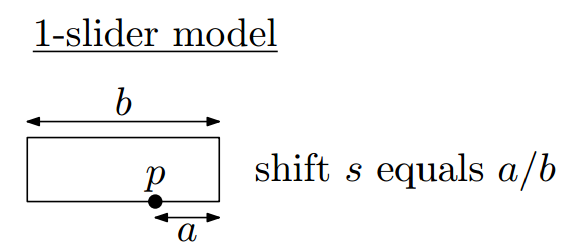
\includegraphics[scale = 0.5]{1slider.png}\\
 \caption{A graphic showing the three placement models}
 \end{figure}
 \end{enumerate}

In section ... we describe the algorithm we have created for the 2-position model which has a running time of $O(n^2)$. In section ... we describe the algorithm we have created for the 4-position model which has a running time of $O(n^2)$. In section ... we describe the algorithm we have created for the 1-slider model which has a running time of ...

\end{document}
